\documentclass[11pt,UTF8]{ctexart}
\usepackage{titling}
\usepackage{enumerate}
\usepackage{amsmath,amssymb,amsfonts}
\usepackage{listings}
\usepackage{comment}
\usepackage{forest}
\usepackage{bm}
\usepackage{float}
\usepackage{graphicx}
\usepackage{multicol,multirow}
\usepackage{bigstrut}
\usepackage[unicode=true,%本行非常重要 支持中文目录hyperref CJKbookmarks对二级目录没用
	colorlinks,
	linkcolor=black,
	anchorcolor=black,
	citecolor=black,
	CJKbookmarks=false]{hyperref}
\usepackage{xcolor}
\usepackage{geometry}
\geometry{top=20mm,bottom=20mm,left=20mm,right=20mm}
\pagestyle{plain}%删除页眉
\CTEXsetup[format={\Large\bfseries}]{section}

\lstset{basicstyle=\small}

\def\toprule{\hline}
\def\midrule{\hline}
\def\bottomrule{\hline}

\setlength{\droptitle}{-50pt}%减少标题与页眉距离

\title{数电实验7报告}
\author{17341015\quad数据科学与计算机学院\\计科一班\quad陈鸿峥}
\date{}

\begin{document}
\maketitle
\vspace{-50pt}%减少标题与正文距离
\lstset{language=C++,escapechar=`}

% 真值表 -> 卡诺图 -> 逻辑表达式 -> 选择器件实现
\section{内容一}
\subsection{实验目的}
验证四位双向移位寄存器74LS194的功能

\subsection{实验原理}
\begin{table}[H]
  \centering
    \begin{tabular}{|c|c|c|c|}
    \hline
    $\overline{Cr}$    & $S_1$    & $S_0$ & 功能 \bigstrut\\
    \hline
    0     & X & X     & 置零 \bigstrut\\
    \hline
    1     & 0 & 0     & 保持 \bigstrut\\
    \hline
    1     & 0 & 1     & 右移 \bigstrut\\
    \hline
    1     & 1 & 0     & 左移 \bigstrut\\
    \hline
    1 & 1 & 1 & 并行送数\\
    \hline
    \end{tabular}%
\end{table}%

\subsection{实验细节}
\subsubsection{实验仪器及器件}
\begin{enumerate}
    \item 数字电路实验箱、示波器、导线若干
    \item 74LS194*1, 74LS197*1
\end{enumerate}

\subsubsection{实验流程}
\begin{enumerate}
    \item 将74LS197连接成十六进制作为电路的输入信号源:$\overline{PL}$,$\overline{MR}$接高电平,CP0接时钟输入
    \item 将74LS194与74LS197相连,观察输出波形
\end{enumerate}

\subsection{结果分析及结论}
\par 静态测试:接01显示器显示正常
\par 动态测试:实验箱连线如下

\par 波形图如下
\begin{figure}[H]
    \centering
    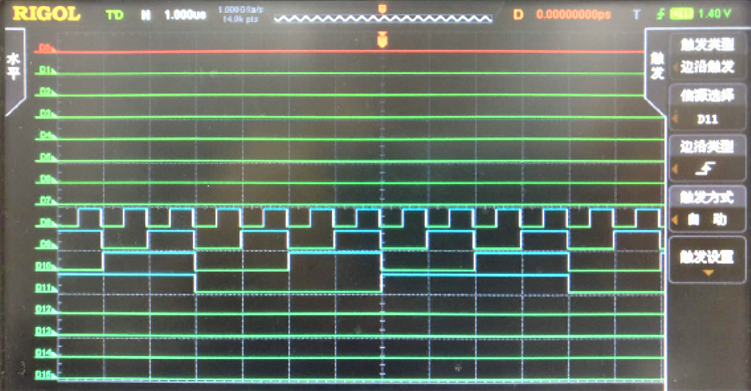
\includegraphics[width=0.9\linewidth]{fig/wave1.PNG}
\end{figure}

\par 从图中可以明显看出分频特性,符合预期


\section{内容二}
\subsection{实验目的}
实现四节拍脉冲发生器

\subsection{实验原理}
将四位双向移位寄存器与JK触发器相连可实现效果,需要注意输入与输出不要连反,实验过程中因为逻辑门的输入输出连反,导致只有两位循环

\subsection{实验细节}
\subsubsection{实验仪器及器件}
\begin{enumerate}
    \item 数字电路实验箱、示波器、导线若干
    \item 74LS194*1, 74LS73*1, 74LS197*1
\end{enumerate}

\subsubsection{实验流程}
\begin{enumerate}
    \item 将74LS197连接成十六进制作为电路的输入信号源:$\overline{PL}$,$\overline{MR}$接高电平,CP0接时钟输入
    \item 将74LS73与74LS194相连,按照书上连线方法将其余导线连接
    \item 用示波器观测并记录波形
\end{enumerate}

\subsection{结果分析及结论}
\par 静态测试:接01显示器显示正常
\par 动态测试:波形图如下
\begin{figure}[H]
    \centering
    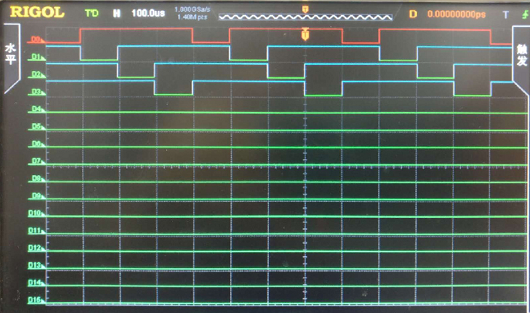
\includegraphics[width=0.9\linewidth]{fig/wave2.PNG}
\end{figure}


\section{内容三}
\subsection{实验目的}
实现扫描译码显示电路

\subsection{实验原理}
通过拨码开关来实现BCD码的输入,并将其传入到译码器中,再将译码器与七段数码管相连. 通过人眼视觉的暂存效应,当时钟频率足够快时,即可正常在数码管上显示数码.


\subsection{实验细节}
\subsubsection{实验仪器及器件}
\begin{enumerate}
    \item 数字电路实验箱、示波器、导线若干
    \item 74LS197*1
    \item 74LS48*1,74LS138*1
\end{enumerate}

\subsubsection{实验流程}
\begin{enumerate}
    \item 将74LS197连接成十六进制作为电路的输入信号源:$\overline{PL}$,$\overline{MR}$接高电平,CP0接时钟输入
    \item 将74LS197的输出与74LS138相连,74LS138的输出与七段数码管的选通位相连
    \item 74LS48与四个拨码开关相连,输出直接与七段数码管相连
\end{enumerate}

\subsection{结果分析及结论}
\par 静态测试:接01显示器显示正常
\par 动态测试:结果上课时已交给助教检查,没有存图,但可以做到通过拨码开关改变数码管的输出,且四位输出相同


\section{内容四}
\subsection{实验目的}
用LED数码管显示8位学号

\subsection{实验原理}
\par 由于我的学号都是在0到7之间,所以只需接通一个74LS197的八进制计数器.
\par 将其输出分别接到74LS48和74LS138,通过选通再加以高频时钟,即可正常实现学号的显示.

\subsection{Protues仿真结果}
\begin{figure}[H]
    \centering
    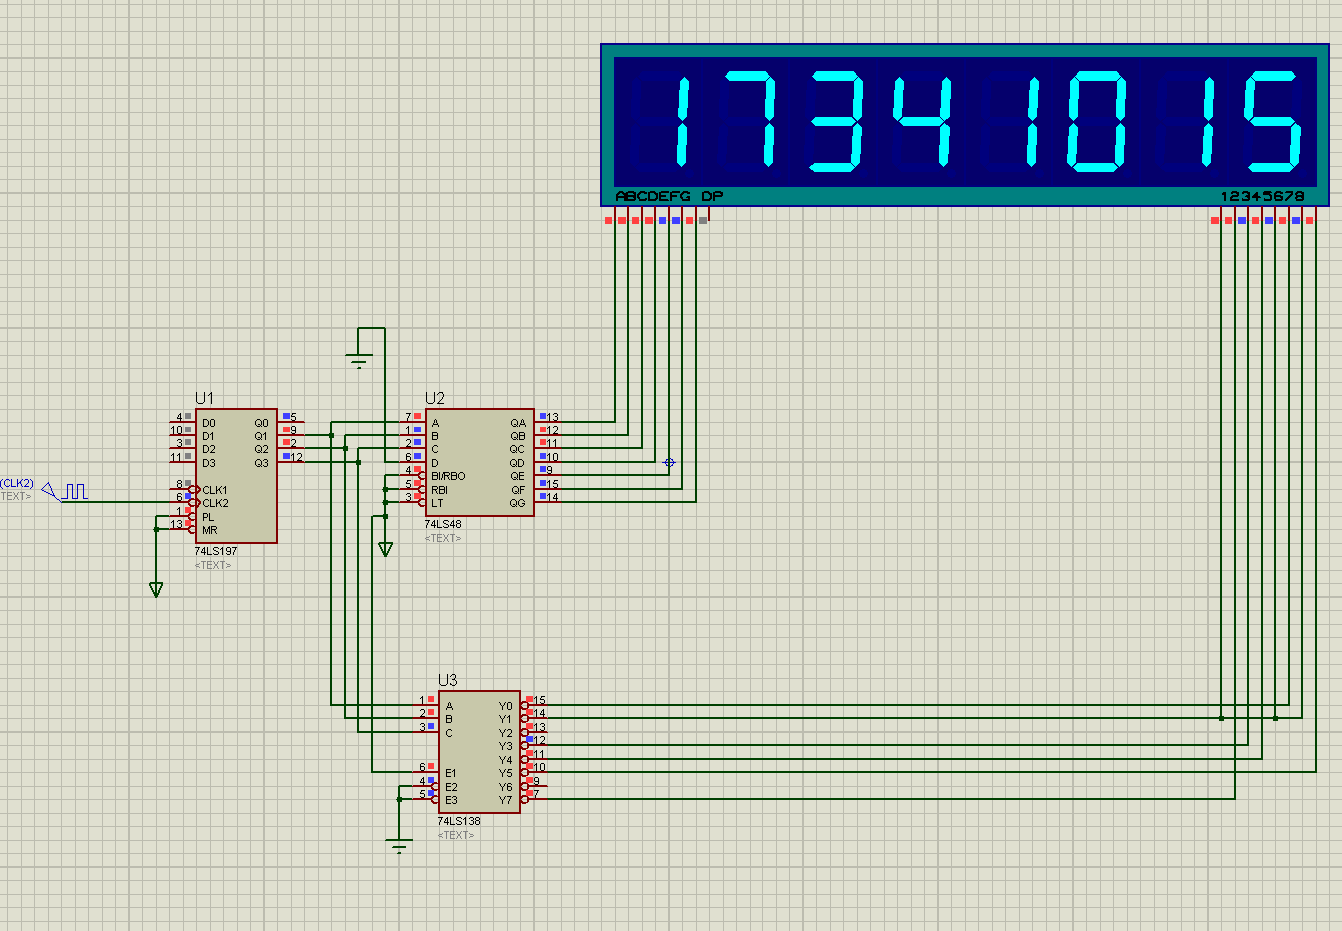
\includegraphics[width=0.9\linewidth]{fig/num.PNG}
\end{figure}


\section{内容五}
\subsection{实验目的}
在点阵面板显示图案

\subsection{实验原理}
点阵的行为高电平,点阵的列为低电平时,对应的点将会亮灯,故可以通过在不同的时间(行)选通不同的列来实现点阵的显示,如数字0的真值表如下
% Table generated by Excel2LaTeX from sheet 'Sheet1'
\begin{table}[H]
  \centering
    \begin{tabular}{|r|r|r|r|r|r|r|r|r|r|r|}
\cline{4-11}    \multicolumn{1}{r}{} & \multicolumn{1}{r}{} &       & 1     & 2     & 3     & 4     & 5     & 6     & 7     & 8 \bigstrut\\
    \hline
    0     & 0     & 0     & 0     & 0     & 0     & 0     & 0     & 0     & 0     & 0 \bigstrut\\
    \hline
    0     & 0     & 1     & 0     & 0     & \textcolor[rgb]{ 1,  0,  0}{1} & \textcolor[rgb]{ 1,  0,  0}{1} & \textcolor[rgb]{ 1,  0,  0}{1} & \textcolor[rgb]{ 1,  0,  0}{1} & 0     & 0 \bigstrut\\
    \hline
    0     & 1     & 0     & 0     & 0     & \textcolor[rgb]{ 1,  0,  0}{1} & 0     & 0     & \textcolor[rgb]{ 1,  0,  0}{1} & 0     & 0 \bigstrut\\
    \hline
    0     & 1     & 1     & 0     & 0     & \textcolor[rgb]{ 1,  0,  0}{1} & 0     & 0     & \textcolor[rgb]{ 1,  0,  0}{1} & 0     & 0 \bigstrut\\
    \hline
    1     & 0     & 0     & 0     & 0     & \textcolor[rgb]{ 1,  0,  0}{1} & 0     & 0     & \textcolor[rgb]{ 1,  0,  0}{1} & 0     & 0 \bigstrut\\
    \hline
    1     & 0     & 1     & 0     & 0     & \textcolor[rgb]{ 1,  0,  0}{1} & 0     & 0     & \textcolor[rgb]{ 1,  0,  0}{1} & 0     & 0 \bigstrut\\
    \hline
    1     & 1     & 0     & 0     & 0     & \textcolor[rgb]{ 1,  0,  0}{1} & \textcolor[rgb]{ 1,  0,  0}{1} & \textcolor[rgb]{ 1,  0,  0}{1} & \textcolor[rgb]{ 1,  0,  0}{1} & 0     & 0 \bigstrut\\
    \hline
    1     & 1     & 1     & 0     & 0     & 0     & 0     & 0     & 0     & 0     & 0 \bigstrut\\
    \hline
    \end{tabular}%
\end{table}%

\subsection{实验结果}
\par 数字与英文在课堂上已交由助教检查,没有存图
\par 数字是一个0字,英文是一个H,下图是数字0的连接电路
\begin{figure}[H]
    \centering
    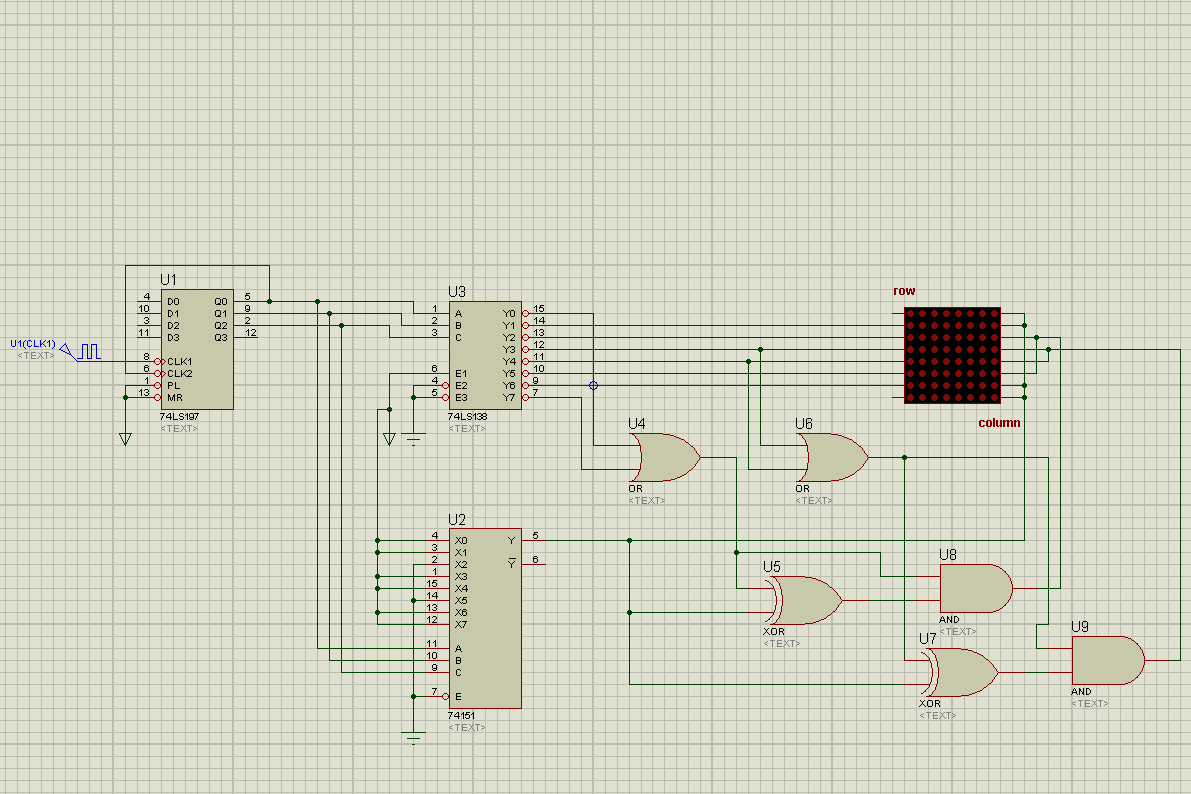
\includegraphics[width=0.9\linewidth]{fig/lattice0.PNG}
\end{figure}
\par 下图是一个旧字
\begin{figure}[H]
    \centering
    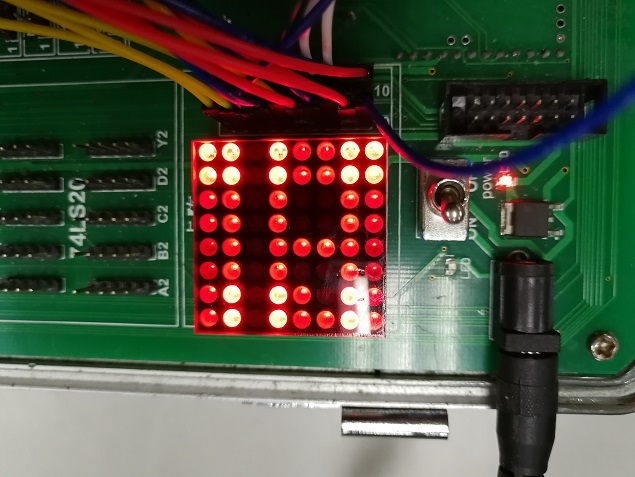
\includegraphics[width=0.9\linewidth]{fig/word.jpg}
\end{figure}


\section{内容六(加分题)}
\subsection{实验目的}
在Basys3实验板上通过拨码开关,分别显示学号的前四位和后四位

\subsection{Bayse板电路实现}
\par Verilog程序如下,学号显示部分
\begin{lstlisting}[language=Verilog]
module display (
    input [1:0] digit,
    input fb,
    output reg [6:0] seven_seg
    );

    // seven segments
    parameter zero  = 7'b000_0001;
    parameter one   = 7'b100_1111;
    parameter two   = 7'b001_0010;
    parameter three = 7'b000_0110;
    parameter four  = 7'b100_1100;
    parameter five  = 7'b010_0100;
    parameter six   = 7'b010_0000;
    parameter seven = 7'b000_1111;
    parameter eight = 7'b000_0000;
    parameter nine  = 7'b000_0100;

    always @(digit)
    if (fb == 1)
    begin
        case(digit)
            0: seven_seg = four;
            1: seven_seg = three;
            2: seven_seg = seven;
            3: seven_seg = one;
        endcase // clk
    end
    else begin
    case(digit)
        0: seven_seg = five;
        1: seven_seg = one;
        2: seven_seg = zero;
        3: seven_seg = one;
    endcase // clk
    end

endmodule
\end{lstlisting}
\par 分频计数器与七段数码管连接部分
\begin{lstlisting}[language=Verilog]
module Counter(
    input clr, // clear, say reset
    input wire clk, // clock
    input wire fb, // front or back
    output [6:0] seg,
    output reg [3:0] an
    );

    reg [1:0] out;
    parameter MAX_COUNT = 4;
    
    // time counter
    localparam MAX_COUNT_TIME = 100_000; // 10kHz
    reg [16:0] count; // 26 bits to store count: 2^17 > 10^5
    always @ (posedge clk or posedge clr)
    begin
        if (clr == 1) // reset
            count <= 0;
        else if (count == MAX_COUNT_TIME - 1) // return 0
            count <= 0;
        else
            count <= count + 1;
    end

    // frequency divisor (flip-flop)
    reg clk_div;
    always @ (posedge clk, posedge clr)
    begin
        if (clr == 1)
            clk_div <= 0;
        else if (count == MAX_COUNT - 1) // reset
            clk_div <= ~clk_div;
        else // set
            clk_div <= clk_div;
    end

    always @ (posedge clk_div or posedge clr)
    begin
        if (clr == 1)
            out <= 0;
        if (out == MAX_COUNT)
            out <= 0;
        else
            out <= out +1;
    end

    display disp1 (.digit(out),.seven_seg(seg),.fb(fb));
    
    always @ (out)
        case(out)
            0: an = 4'b1110;
            1: an = 4'b1101;
            2: an = 4'b1011;
            3: an = 4'b0111;
        endcase

endmodule
\end{lstlisting}
\par 限制文件如下
\begin{lstlisting}[language=Verilog]
set_property PACKAGE_PIN W4 [get_ports {an[3]}]
set_property PACKAGE_PIN V4 [get_ports {an[2]}]
set_property PACKAGE_PIN U4 [get_ports {an[1]}]
set_property PACKAGE_PIN U2 [get_ports {an[0]}]
set_property PACKAGE_PIN W7 [get_ports {seg[6]}]
set_property PACKAGE_PIN W6 [get_ports {seg[5]}]
set_property PACKAGE_PIN U8 [get_ports {seg[4]}]
set_property PACKAGE_PIN V8 [get_ports {seg[3]}]
set_property PACKAGE_PIN U5 [get_ports {seg[2]}]
set_property PACKAGE_PIN V5 [get_ports {seg[1]}]
set_property PACKAGE_PIN U7 [get_ports {seg[0]}]

set_property PACKAGE_PIN W5 [get_ports clk]
set_property IOSTANDARD LVCMOS33 [get_ports {an[3]}]
set_property IOSTANDARD LVCMOS33 [get_ports {an[2]}]
set_property IOSTANDARD LVCMOS33 [get_ports {an[1]}]
set_property IOSTANDARD LVCMOS33 [get_ports {an[0]}]
set_property IOSTANDARD LVCMOS33 [get_ports {seg[6]}]
set_property IOSTANDARD LVCMOS33 [get_ports {seg[5]}]
set_property IOSTANDARD LVCMOS33 [get_ports {seg[4]}]
set_property IOSTANDARD LVCMOS33 [get_ports {seg[3]}]
set_property IOSTANDARD LVCMOS33 [get_ports {seg[2]}]
set_property IOSTANDARD LVCMOS33 [get_ports {seg[1]}]
set_property IOSTANDARD LVCMOS33 [get_ports {seg[0]}]
set_property IOSTANDARD LVCMOS33 [get_ports clk]

set_property PACKAGE_PIN V17 [get_ports clr]
set_property PACKAGE_PIN R2 [get_ports fb]
set_property IOSTANDARD LVCMOS33 [get_ports clr]
set_property IOSTANDARD LVCMOS33 [get_ports fb]
\end{lstlisting}
\par 最终结果图如下
\begin{figure}[H]
    \centering
    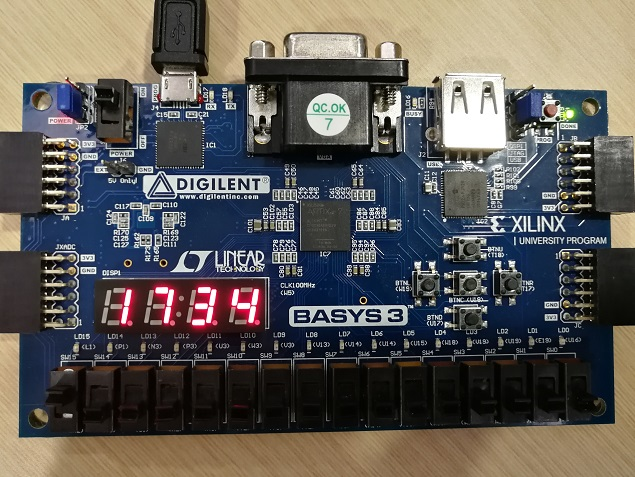
\includegraphics[width=0.8\linewidth]{fig/b1.jpg}
\end{figure}
\begin{figure}[H]
    \centering
    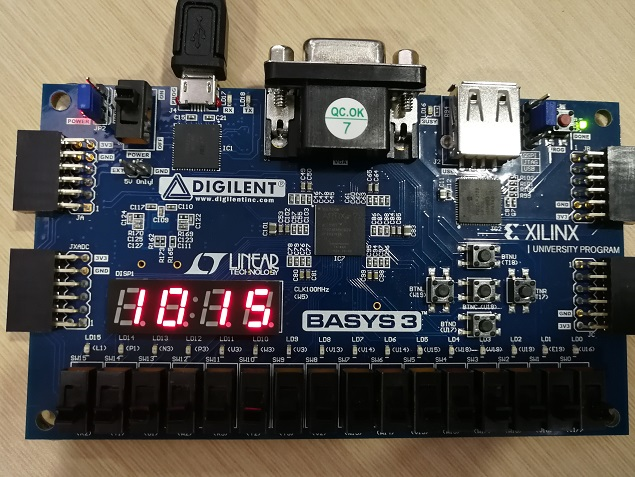
\includegraphics[width=0.8\linewidth]{fig/b2.jpg}
\end{figure}

\section{心得体会}
\begin{enumerate}
    \item 学会了移位寄存器及JK触发器的使用及其功能
    \item 明白译码显示电路的原理,并将其实际运用起来
    \item 更好地学会用Verilog进行电路设计分析,并成功上板实现
\end{enumerate}


\end{document}